\section{研究方法}
\subsection{模型讨论}
\par 经典SIR模型的表述方式简洁直观,但在扩建模型时会有一些繁琐:
由表\ref{table:SIR模型符号表}可预见,随着划分人群的增多,人群间感染机制也随之复杂,不同人群之间转变率的符号也会增多或者改变含义,这会使读者对符号的理解产生负面的路径依赖影响,对于模型的扩建是十分不利的。
\par 本文将采用另一种较为抽象的模型表述方式,以此来减轻读者的思维负担。
\begin{table}[H]
    \centering
    \caption{另一种模型符号表示}
    \begin{tabular}{ll}
        \hline
        符号       & 含义                              \\
        \hline
        $\P{a}{b}$ & a群体变为b群体的概率              \\
        $\T{a}{b}$ & 单位时间$t$内a群体变为b群体的人数 \\
        \hline
    \end{tabular}
\end{table}
\par 将a到b群体的转换概率用$\P{a}{b}$表示,单位时间内a到b群体转变的人数为$\T{a}{b}$。
\par 感染机制如下:
\begin{align}
    S(t)\xrightarrow{\P{S}{I}}I(t) \Rightarrow \TP{S}{I}{SI} \\
    I(t)\xrightarrow{\P{I}{R}}R(t) \Rightarrow \TP{I}{R}{I}
\end{align}
\par 可将其简化为:
\begin{align}
    \TP{S}{I}{SI} \\
    \TP{I}{R}{I}
\end{align}
\par 将所有人群放到一个集合$\mathbb{A}$中,则模型的积分方程为:
\begin{equation}
    \dt{a} = \sum\left(\T{b}{a}-\T{a}{b}\right)
\end{equation}
\par 其中$a\in\mathbb{A}$,$b\in\mathbb{A}$且$b\not=a$,不在感染机制中的$\T{a}{b}$为$0$。
\par 该积分式对本文中提到的所有模型都适用,
读者不必再关心模型的积分式,
只需关注模型新引入的群体及其引起的感染机制$\T{a}{b}$变化即可
(详细积分式仍会给出,以便深入理解模型的变化)。
\par 现在,可以仅通过感染机制来方便清晰的描述$SIR$模型:
\begin{align}
    \TP{S}{I}{SI} \\
    \TP{I}{R}{I}
\end{align}
\subsection{模型推论}
\par 本文共引入$5$种人群,在此声明。
\begin{table}[H]
    \centering
    \caption{人群}
    \begin{tabular}{ll}
        \hline
        符号 & 含义   \\
        \hline
        $S$  & 易感者 \\
        $I$  & 感染者 \\
        $R$  & 康复者 \\
        $E$  & 携带者 \\
        $D$  & 病逝者 \\
        \hline
    \end{tabular}
\end{table}
\subsubsection{$SEIR$模型}
\par 考虑到易感人群接触到感染者后不会立即患病,
而是经过一段时间潜伏期,
即携带病毒还未患病,
将该类人群定义为携带者人群$E$,
该人群有可能转变为治愈者$R$或感染者$I$,
即为$SEIR$模型。
在COVID-19中这类人群一般会通过检测试剂等方式被诊断为疑似病例。
\subsubsection{感染机制}
\begin{align}
    \TP{S}{E}{S(I+E)} \\
    \TP{E}{R}{E}      \\
    \TP{E}{I}{E}      \\
    \TP{I}{R}{I}
\end{align}
\subsubsection{详细积分式}
\SEIR
\subsubsection{$SEIRD$模型}
\par 在$SEIR$的基础上加入死亡人群$D$,
即为$SEIRD$模型。
\subsubsection{感染机制}
\begin{align}
    \TP{S}{E}{S(I+E)} \\
    \TP{E}{R}{E}      \\
    \TP{E}{I}{E}      \\
    \TP{I}{R}{I}      \\
    \TP{I}{D}{I}
\end{align}
\subsubsection{详细积分式}
\SEIRD
\subsubsection{$SEIRS$模型}
\par 考虑到治愈者有复发的可能,
康复者有一定比例重新转变为感染者,
加入新的传播机制$\T{R}{I}$,
即为$SEIRS$模型。
\subsubsection{感染机制}
\begin{align}
    \TP{S}{E}{S(I+E)} \\
    \TP{E}{R}{E}      \\
    \TP{E}{I}{E}      \\
    \TP{I}{R}{I}      \\
    \TP{I}{D}{I}      \\
    \TP{R}{I}{R}
\end{align}
\subsubsection{详细积分式}
\SEIRS
\subsection{对隔离的处理}
\par 本文并未尝试引入隔离群体的$SEIHR$模型,
因为在该数据中隔离群体是携带者、感染者的混合群体,
且隔离群体有可能治愈或死亡,
而这其中的比例无法通过现有数据得知,
故不能通过拟合来确定其参数。
\par 对于隔离的处理,
本文将数据分为隔离前与隔离后两部分,
对这两个时间段的数据分别进行拟合,
以此来对比隔离前后对疫情传播的影响。
\subsection{数据拟合结果及分析}
\par 拟合所用数据为2020年1月20日至5月1日官方发布的全国疫情数据。
以下为官方发布的疫情数据:
\\
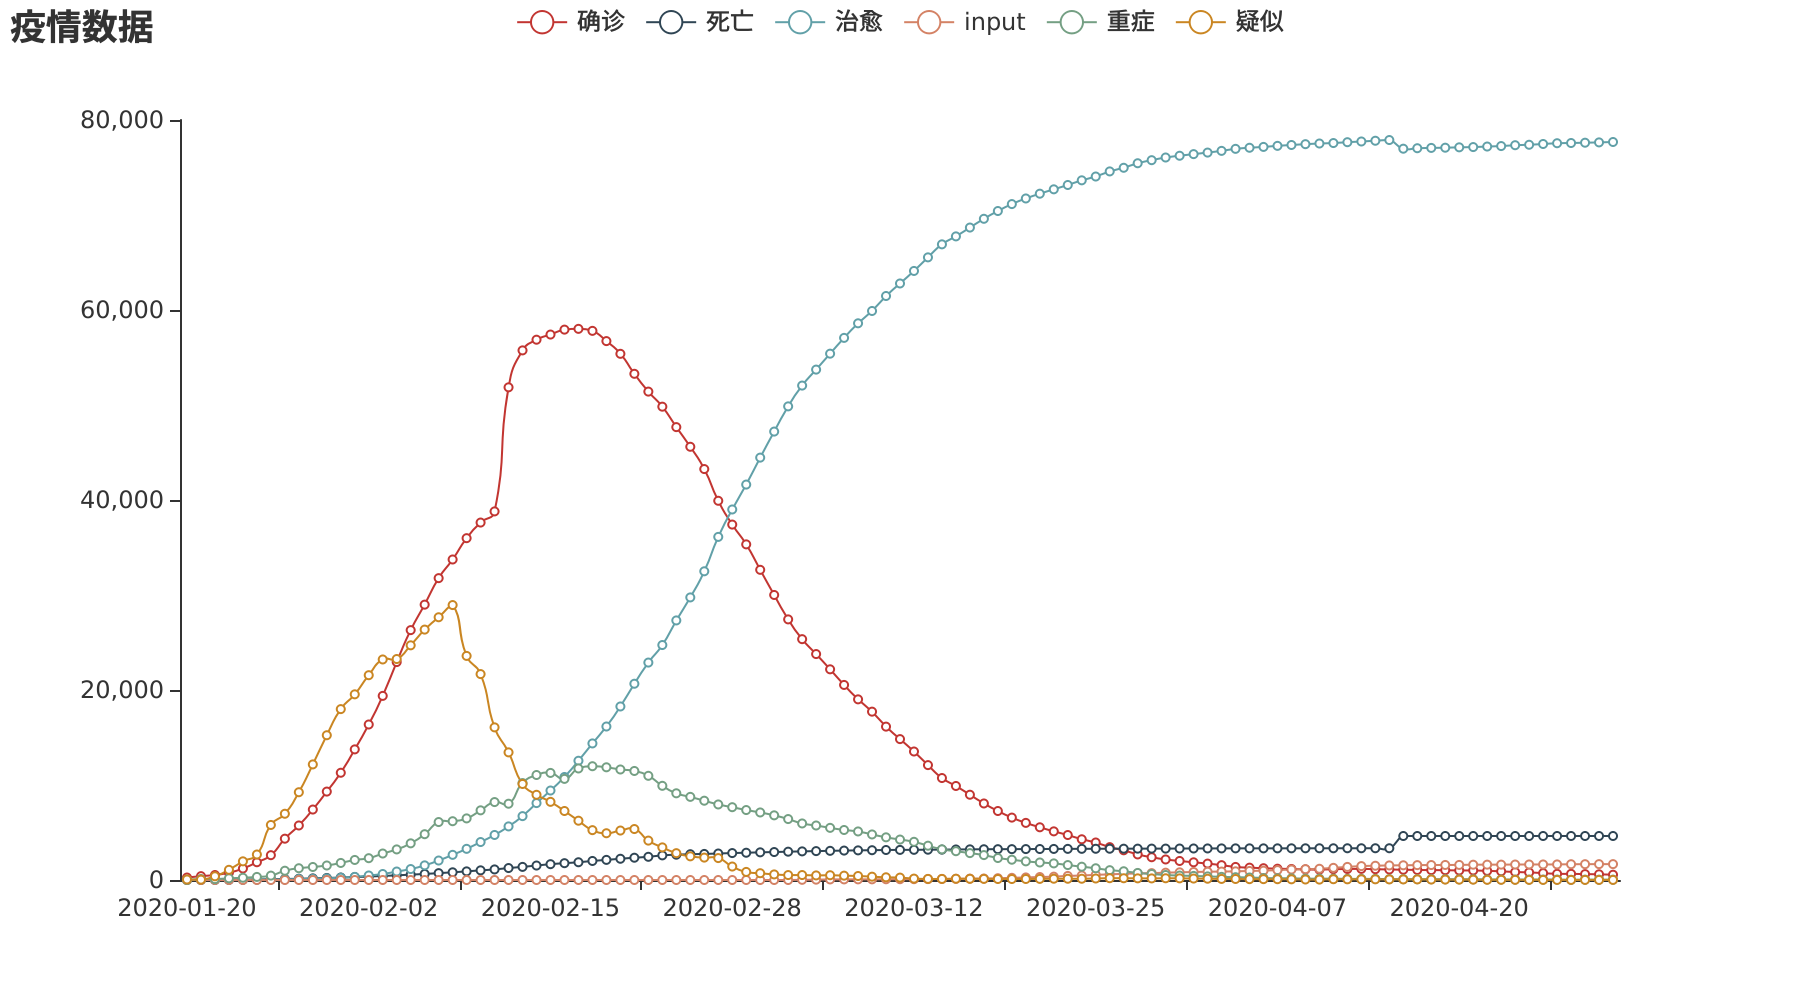
\includegraphics[width=\imagewidth]{疫情数据.png}
\\
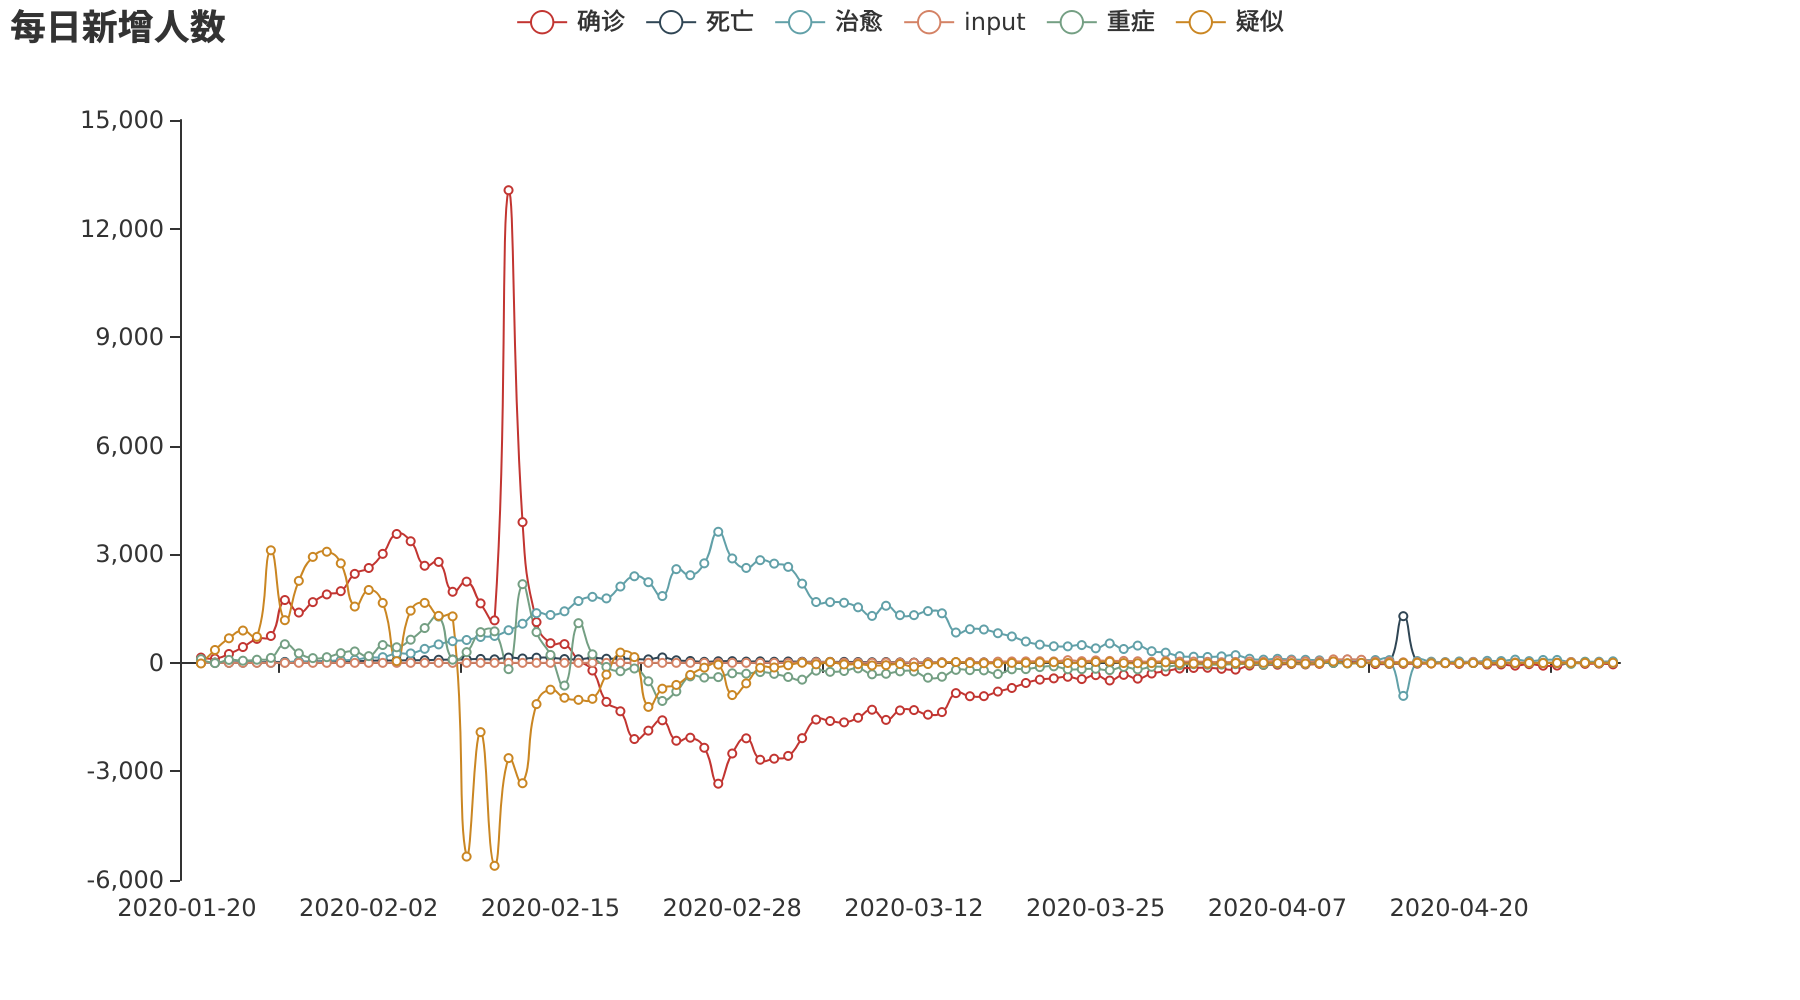
\includegraphics[width=\imagewidth]{每日新增人数.png}
\par
2月12日确诊人数猛增,
是因为当日重新规定了确诊条件,
导致许多疑似病例纳入确诊人数。
\par 本文采取$L-BFGS-B$方法对每个模型进行拟合,
将每个模型的预测值与真实数据进行对比,
并给出拟合后的参数以及损失值$LOSS$,
损失值将作为评判模型拟合优劣的指标之一。
\par 损失值定义:
\begin{equation}
    LOSS = \frac{\sum\limits^{day}\sum\limits^{group}
        \left|True-Predict\right|}{day}
\end{equation}
\par 对比各个模型间的$LOSS$值:
\showtable{SIR}
\par $SIR$模型中$\P{S}{I}$为感染人数增长率,
不同于感染率。
$\P{I}{R}$为治愈人数增长率,
不同于治愈率。
\showtable{SEIR}
\par $SEIR$模型中$\P{E}{R}$极低,
一可理解为潜伏期较长,
二可理解为致病率较高,
这两点都与实际情况吻合。
\showtable{SEIRD}
\par $SEIRD$模型中$\P{I}{D}$为死亡人数增长率,
不同于死亡率。
\showtable{SEIRS}
\par $SEIRS$模型中的$\P{R}{I}=0.001$,
可以理解为复阳率极低,
说明复阳人数占患病人数比例极低,
对疫情的影响微乎其微。
\par 仅从$LOSS$值判断,
模型从优到劣排序为$SEIRD>SEIRS>SEIR>SIR$。
\par 对比各个模型拟合前后的参数值变化:
\showtables{SIR}
$\P{S}{I}$有所下降,
$\P{I}{R}$有所增减,
代表感染率降低,
治愈率提高。
\showtables{SEIR}
$\P{S}{E},\P{E}{I}$有所下降,
$\P{I}{R}$有所增减,
代表感染率降低,
治愈率提高。
\showtables{SEIRD}
$\P{S}{E}$稍有增加,
$\P{E}{I}$有所下降,
$\P{S}{E}\cdot \P{E}{I}$有所下降,
$\P{I}{R}$有所增减,
$\P{I}{D}$有所下降
代表患病率降低,
治愈率提高,
死亡率降低。
\showtables{SEIRS}
$SEIRS$模型与$SEIRD$模型的参数十分接近,
无论分段与否,$SEIRS$模型的$\P{S}{I}$均为$0.001$,
说明$\P{S}{I}$对模型的影响极其微弱,
判断可以将$\T{S}{I}$从模型中剔除,
并参考$LOSS$值的大小,
认为在上述几种模型中,
$SEIRD$模型最适用于该类传染病预测。
\par 无论哪种模型,
比较模型分段前后参数,
均可得出传染病的传染率降低、治愈率增加、死亡率降低这一结论,
可以说明隔离措施十分有效。
\par 根据$SEIRD$模型的拟合参数,
可以计算出病毒大致的基础再生数
$R_0$\cite{应用SEIR模型预测2009年甲型H1N1流感流行趋势,王宝童2013流感传播数学模型的基本再生数}:
\begin{equation}
    R_0 = \frac{\P{S}{I}}{\P{I}{R}}
    = \frac{\P{S}{E}\cdot \P{E}{I}}{\P{I}{R}}
\end{equation}
\par 计算出隔离前$R_0=5.937$,隔离后$R_0=1.242$,可见疫情传播得到了有效的抑制。